% !TEX root = MutationTestingSurvey.tex

\section{Mutation Testing Process}
\label{sec:dataProcess}

	\begin{figure}
	\centering
		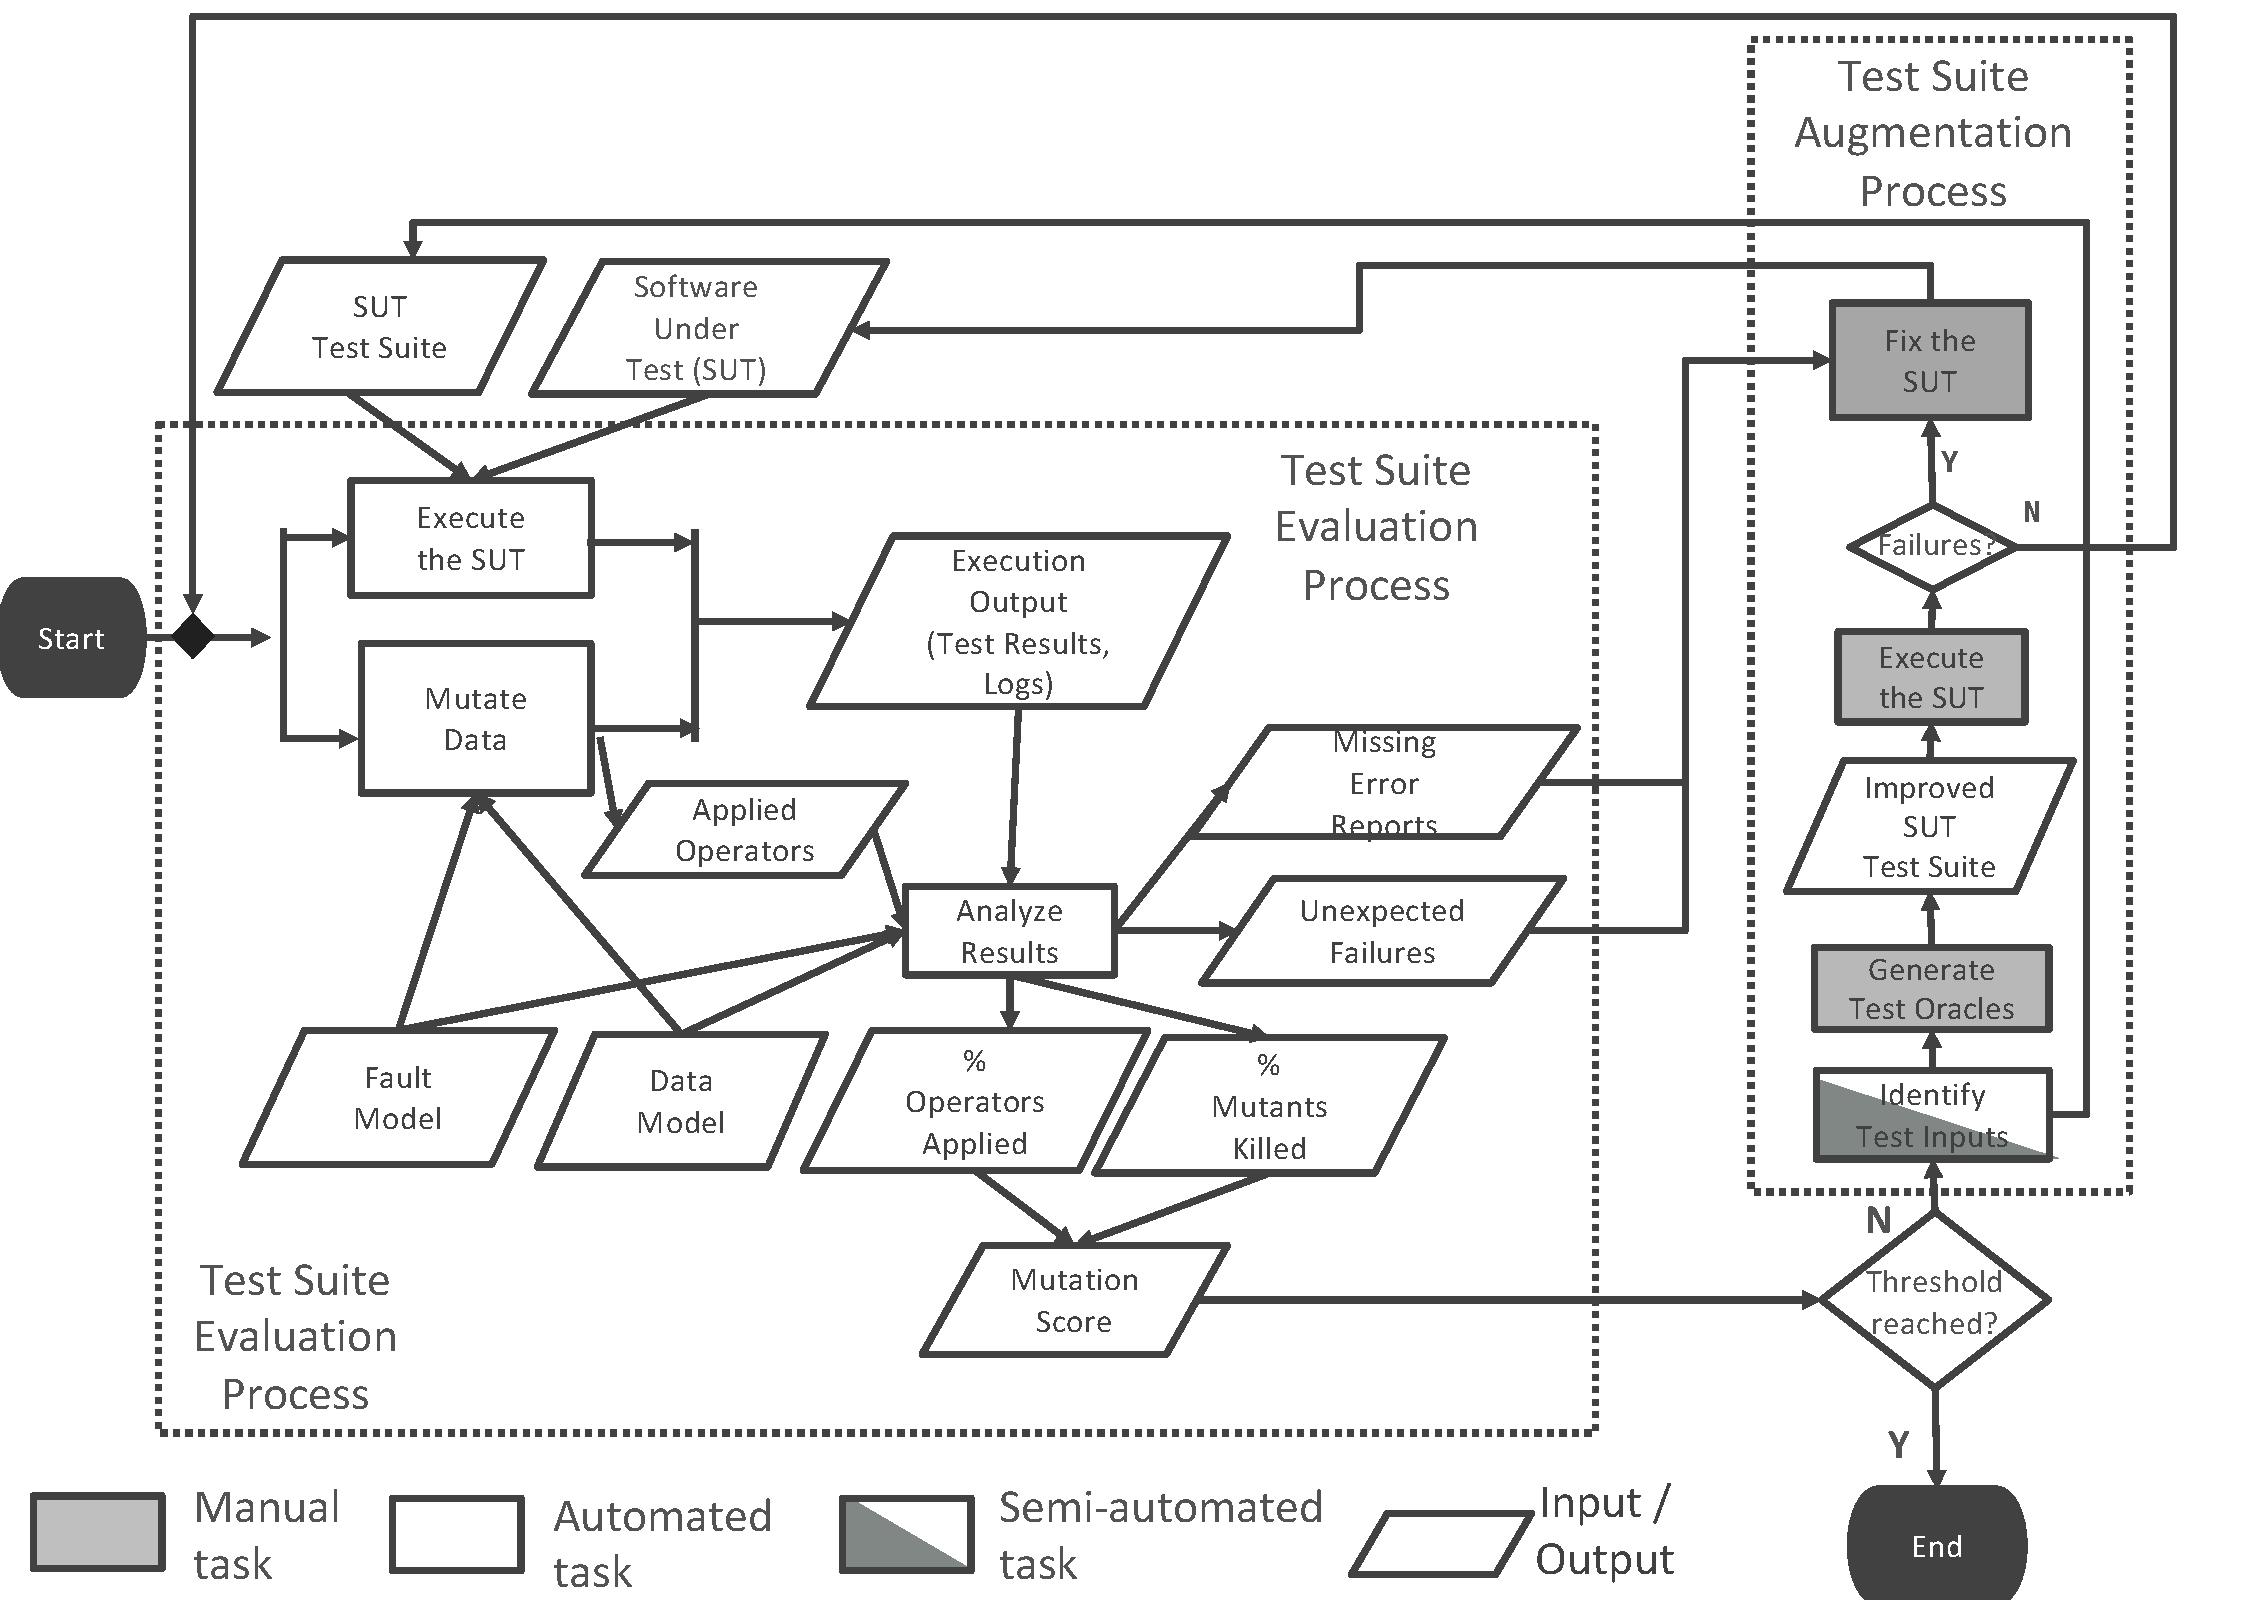
\includegraphics[width=\textwidth]{images/dataProcess}
		\caption{Data-driven Mutation Testing Process.}
		\label{fig:data:process}
	\end{figure}



This Chapter is a first attempt towards the formalization of a test suite assessment process based on the injection of faults in the data processed by software components; we refer to this process as \emph{data-driven mutation testing}. 

Data-driven mutation testing aims to assess test suites by simulating faults that affect the data produced, received, or exchanged by the software and its components.
It is based on a \INDEX{fault model} capturing the type of data faults that might affect the system. The fault model is produced by software engineers based on their domain knowledge and experience~\cite{di2015generating}. \MREVISION{C18}{The considered faults might be due to programming errors, hardware problems, or critical situations in the environment (e.g., noise in the channel).} The data is the automatically mutated by a set of operators that aim to replicate the faults in the fault model. A simple operator is the \INDEX{bit flip operator}, which could be implemented through a procedure that flips a randomly selected bit of every field of the transmitted data (see Section~\ref{sec:data_operators}).


Figure \ref{fig:data:process} shows the reference data-driven mutation testing process that will be considered in this book. The process is based on two main sub-processes, \EMPH{test suite evaluation} and \EMPH{test suite augmentation}, which are described in Sections~\ref{sec:data:test_suite_evaluation}~and~\ref{sec:data:test_suite_augmentation}, respectively. Differently from the code-driven mutation testing process introduced in Section~\ref{sec:process}, the data-driven mutation testing process has not been formalized by existing software testing literature. 
Techniques to inject data faults in the data processed by software systems have been applied mostly to test software systems (e.g., to determine if the software is robust against errors in the data being processed) but not to assess the quality of test suites.
For systems, or components, exchanging structured data (e.g., message sequences), a data fault may consist of either an invalid data structure (i.e., a structure that does not respect the data model of the system) or an illegal data value.
For systems, or components, processing signals, a data fault may result in signals that do not respect the characteristics observed in the original signal. Example of signal features are value, derivative, second derivative~\cite{Matinnejad19}.

Since data-driven mutation testing alters the data produced, received, or exchanged by the software or its components, it should be applied to evaluate test suites that trigger the execution and communication between multiple components (e.g., system or integration test cases). Data-driven mutation testing is not meant to be applied to assess unit test suites.

\subsection{Test Suite Evaluation} % (fold)
\label{sec:data:test_suite_evaluation}

The test suite evaluation process consists of three activities \EMPH{Execute the SUT}, \EMPH{Mutate Data},  and \EMPH{Analyze Results}.
The activity \INDEX{Execute the SUT} indicates that the SUT is executed against its automated test suite. 
The activity \INDEX{Mutate Data} concerns the automated modification of either the data received by the software, the data produced by the software, or the data exchanged by software components.
In Figure~\ref{fig:data:process}, the activity \EMPH{Mutate Data} is executed in parallel to the activity \EMPH{Execute the SUT} since data modification should occur at runtime during test cases execution, to simulate software faults affecting the data processed by the software.

The activity \EMPH{Mutate Data} may require a \INDEX{data model} that captures the characteristics and structure of the data to be mutated. 
For example, the data model is used to load a stream of bytes in structured form (e.g., an instance of a given data structure), which is necessary to drive the data mutation. 
The activity \EMPH{Mutate Data} should be driven by a \INDEX{fault model} that specifies the set of mutation operators to apply~\cite{di2015generating}. 
%The fault model enables engineers to minimize the presence of equivalent mutants.
%The data model may capture the relation between inputs and outputs of the system

Figure~\ref{fig:data:mutateData} provides an example of how the Mutate Data activity can be implemented. Figure~\ref{fig:data:mutateData} shows that, to implement data mutation, it is necessary to integrate additional components that alter the data exchanged by the SUT and its components at runtime on a certain communication layer. Such components can be installed either on the channel or they might be integrated at the boundaries of the software (e.g., by modifying API functions to redirect calls to the mutating component before computing the expected computation).

	\begin{figure}
	\centering
		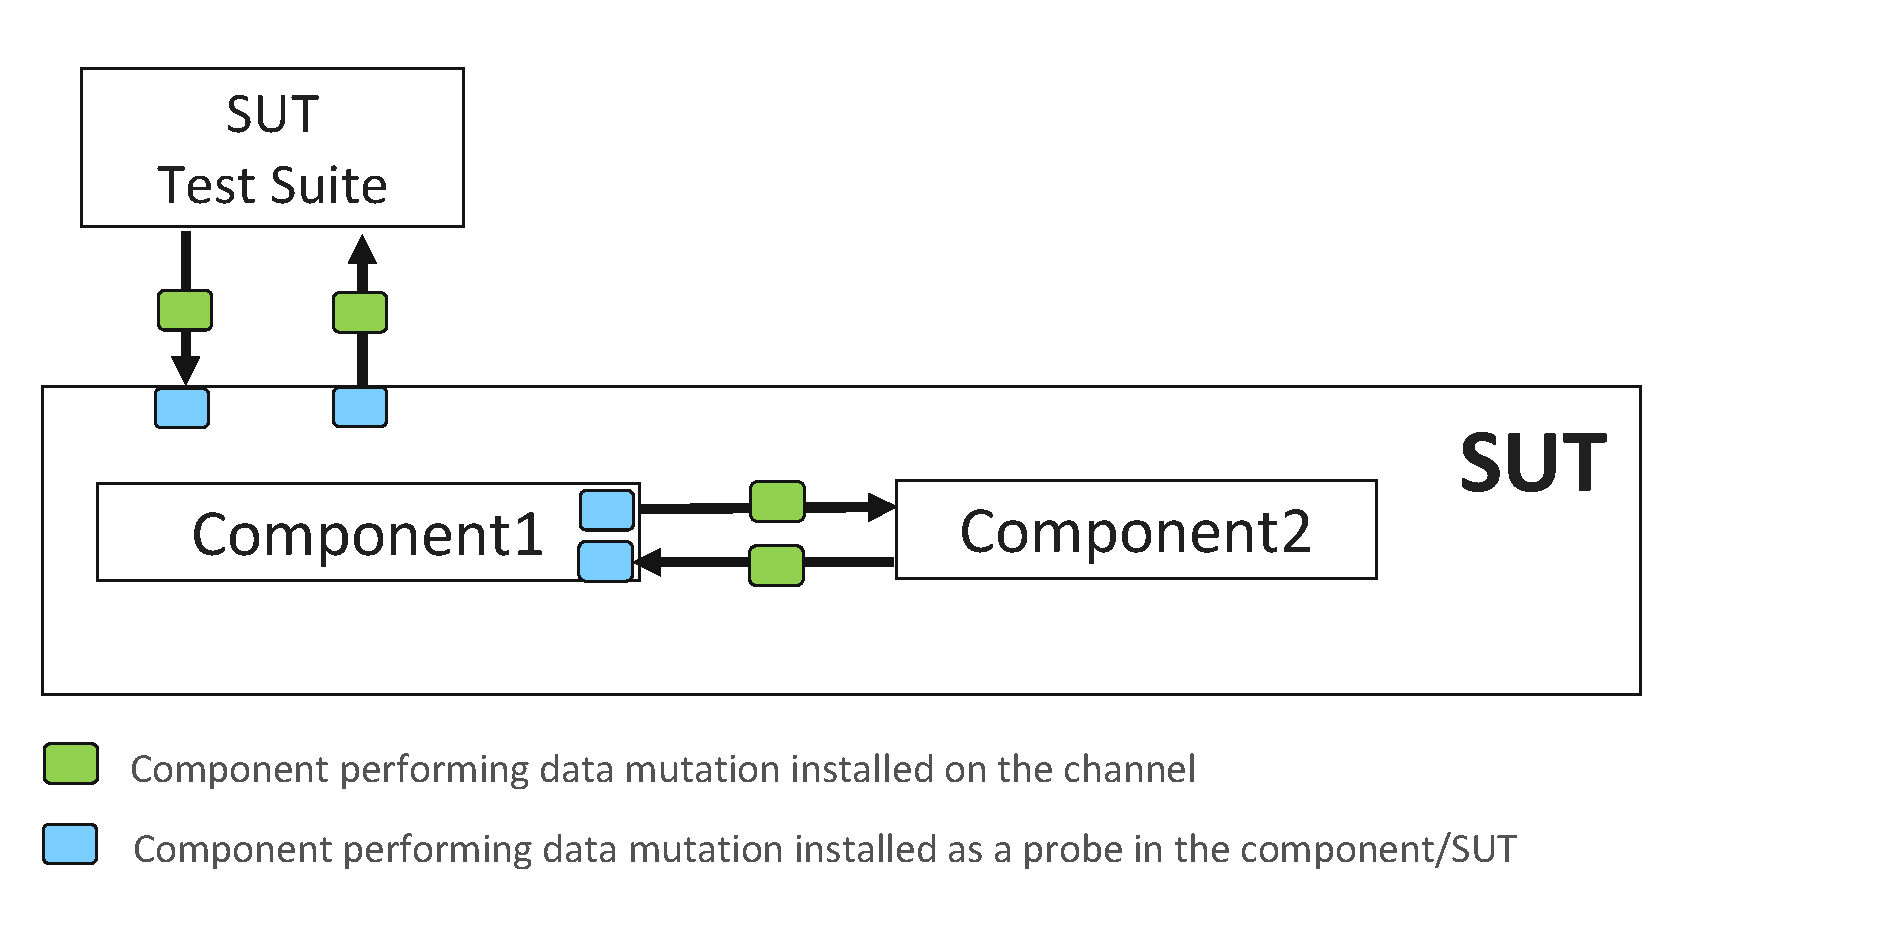
\includegraphics[width=10cm]{images/dataMutationExample}
		\caption{Example of implementation of a data mutation solution.}
		\label{fig:data:mutateData}
	\end{figure}


The activity \INDEX{Analyze Results} processes all the outputs generated during the execution of test cases.
The collected outputs include the result of test cases execution (i.e., the list of test cases that either passed or failed) and the logs generated by the SUT during testing.
In the context of data-driven mutation testing both the \INDEX{test results} and \INDEX{log files} are necessary to determine if a test suite kills a mutant.
Indeed, \emph{in the context of data-driven mutation testing a mutant is killed either if a test case fail, or if the software activates robustness features capable of handling the specific data fault.}
We need log files to determine if robustness features had been triggered.
For example, a system that implements a \INDEX{robust communication protocol} might simply request again the packets affected by errors thus avoiding failures. In this case, we need to inspect the log files to determine if the robustness features had been triggered.

Since data-driven mutation testing does not alter the software implementation but only the data processed by components, it may help engineers to identify existing faults. 
This is the case when \emph{Missing Error Reports} or \emph{Unexpected Failures }(e.g, crashes) are observed. In both the two cases, engineers should fix the system.

The activity Analyze Results provides an assessment of the quality of the test suite for the SUT.
It is driven by two objectives:
\begin{itemize}
\item[(O1)] determine if the test suite is capable of detecting software faults that affect the data processed by the software components 
(e.g., we expect a test suite to fail in case the data exchanged by two components contains invalid values).
\item[(O2)] determine if the test suite exercises enough software behaviours to discover all the possible faults that may affect the data produced by the system
(i.e., it should be possible to alter the processed data to generate faulty data according to the fault model). 
\end{itemize}

\MREVISION{C19}{Objectives O1 and O2 are complementary, \REVTWO{C34}{they both should be addressed by data mutation.}
For example, a use case scenario for data-driven mutation testing could be the following: (i) data-driven mutation testing is applied to the data exchanged by \emph{component 1} and \emph{component 2} in Figure~\ref{fig:data:mutateData}, (ii) the data exchanged by the two components follow the data model in Figure~\ref{fig:DataDrivenSimpleExample}, and (iii) mutation testing is performed by applying the bit-flip mutation operator to every field of the messages being exchanged.
The data model in Figure~\ref{fig:DataDrivenSimpleExample} consists of a UML class diagram that indicates that the two components can send messages whose type can be either \emph{TimeMessage} or \emph{DataMessage}. A \emph{TimeMessage} contains only one field of type Long, which is the timestamp. 
A \emph{DataMessage} contains two fields, one field of type \emph{Integer} capturing the size of the payload, and one array of bytes containing the payload. 
Objective O1 is fulfilled when at least one test case fail for every mutant being created.
Objective O2 is fulfilled when mutation testing generates at least (i) one \emph{TimeMessage} with field \emph{timestamp} being altered,
(ii) one \emph{DataMessage} with field \emph{size} being altered,
and (iii) one \emph{DataMessage} with field \emph{payload} being altered.
For a test suite consisting of two test cases that trigger the exchange of the messages as in the bottom-left part of Figure~\ref{fig:DataDrivenSimpleExample}, the execution of the bit flip mutation operator may lead to messages that lead to test failures. Since all the mutants are killed (i.e., the two test cases fail), objective O1 is achieved. However, the test suite does not lead to the exchange of any message of type \emph{DataMessage}, for this reason objective O2 is not achieved. Objective O2 enables us to determine that the test suite does not excercise the case in which the two components exchange messages of type \emph{DataMessage}. When data-driven mutation testing is performed against components that are expected to guarantee robustness against the exchange of erroneous data, as a by-product, objective O2 also ensures that components robustness is properly tested.}



\REVTWO{C34}{Activity \emph{Analyze Results} concerns the automated computation of the \INDEX{mutation score} from execution data. It is 
computed as the weighted average of the percentage of mutants being killed and the percentage of mutation operators applied.}
The former enables data-driven mutation to achieve objective O1 in Section~\ref{sec:dataProcess}, the latter objective O2. 
Details are provided in Section~\ref{sec:data:mutationscore}.

\REVTWO{C34}{Activity \emph{Analyze Results} takes as input the SUT outputs,  the data model, the fault model, and the list of mutation operators applied.
In the presence of a mutation toolset capable of parsing these files and loading their data as instances of a given data model, this activity can be fully automated.}
The fault model and the data model are used to distinguish between 
data faults that affect the SUT output (i.e., lead to test failures) and
data faults that should be transparently handled by the software (i.e., lead to error messages in the log).
For example, the data model may indicate in which cases an error message should be reported~\cite{di2015generating}.
The list of applied mutation operators should enable engineers to determine if all the available mutation operators have been applied.


\begin{figure}[t!]
  \centering
    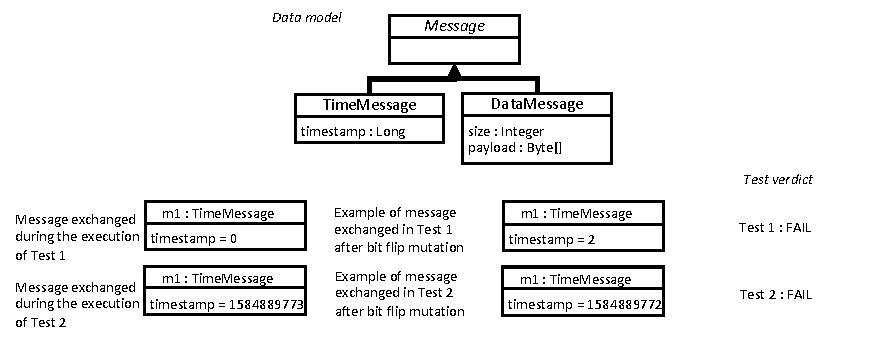
\includegraphics{images/DataDrivenSimpleExample}
      \caption{Simplified data mutation example.}
      \label{fig:DataDrivenSimpleExample}
\end{figure}


The main \INDEX{limitations of data-driven mutation testing} concern: 
\begin{itemize}
\item \MREVISION{C29}{the costs related to data modelling, which is often time consuming.}
\item \MREVISION{C28.a, C28.b}{the necessity of mutating data at runtime, which requires the implementation of probes for the SUT and may lead to increased test execution time. Increased execution time, in turn, may conflict with real-time requirements and may thus force engineers to implement additional optimizations (e.g., offline generation of mutated data).}
\item \MREVISION{C29}{the costs related to fault modelling, which are due not only to the identification of the possible faults that might affect the system but also to the identification and modelling of the possible consequences of the distinct faults (i.e., test failures or triggering of redundancy mechanisms).}
\item \MREVISION{C28.c}{the necessity for processing multiple system outputs, which makes data-driven mutation testing more difficult to integrate in a testing process}.
\item \MREVISION{C28.c}{the presence of equivalent and redundant mutants, which may affect the representativeness of the computed mutation score} \REVTWO{C34}{(see Section~\ref{sec:dataequivalent} for examples)}.
\end{itemize}

In Section~\ref{sec:limitationsData}, we present solutions to address the above-mentioned limitations.

% subsection test_suite_evaluation (end)

\subsection{Test Suite Augmentation} % (fold)
\label{sec:data:test_suite_augmentation}

The test suite augmentation process concerns the definition of additional test cases to increase the mutation score.
It consists of four activities \emph{Identify Test Inputs}, \emph{Generate Test Oracles}, \emph{Execute the SUT}, \emph{Fix the SUT}. 
Despite these activities match the ones performed in the case of code-driven mutation testing, they are triggered and implemented in a different manner, as described below.

%The first two activities concern the definition of new test cases and the improvement of existing test cases.



In the presence of mutants not killed by test cases (i.e., when the \emph{\% of Mutants Killed} is not equal to 100\%), engineers are expected to improve the oracles of existing test cases. Indeed, the presence of mutants not killed by test cases indicates that the oracles of the test suite are not capable of detecting that the software is failing. 
Automated approaches for performing this activity in the presence of system or integration test suites are not available and thus it needs to be performed manually.

In the presence of operators not being applied (i.e., the \emph{\% Operators Applied} is not equal to 100\%), engineers are expected to generate new test inputs for the SUT that enable the application of all the mutation operators. 
For example, in the case of the example in Figure~\ref{fig:DataDrivenSimpleExample}, engineers would need to implement test cases that trigger the exchange of \emph{DataMessages}.
Another example is that of components that exchange message sequences, in the case the test suite trigger only the exchange of message sequences containing only one message. 
Indeed, in this situation, the mutation operator concerning the swapping of two packets cannot be applied. In this case, to achieve 100\% of Operators Applied, engineers should generate inputs that enable the application of the mutation operator (e.g., inputs that lead to a sequence of packets containing more than one packet). 
Fully automated approaches to achieve this objective are unavailable; however, techniques that generate input data from scratch~\cite{gligoric2010test} or augment input data~\cite{DiNardo:TOSEM:2017} can be adopted. 
Also, when the data used by test cases is generated by simulators, meta-heuristic search can be used to drive the generation of input data~\cite{Abdessalem:ICSE:2018}. 

The execution of the SUT and the repair of the SUT are performed manually as in the case of code-driven data mutation.




Section~\ref{sec:testGenerationData} provides details about the existing solutions to  \emph{Identify Test Inputs} and \emph{Generate Test Oracles}.



%
%In this book we focus on the techniques that can be applied to automate the first two activities (i.e., \emph{Identify Test Inputs}, and \emph{Generate Test Oracles}).
% 
%The identification of test inputs has the objective of identifying inputs for the SUT that make the SUT produce an output that is different than the one produced by one of the mutants not killed by the existing test suite.
%
%
%Section~\ref{sec:data:testGeneration} provides an overview of approaches for the automated generation of test cases.

% subsection test_suite_augmentation (end)
